15. \begin{figure}[ht!]
\center{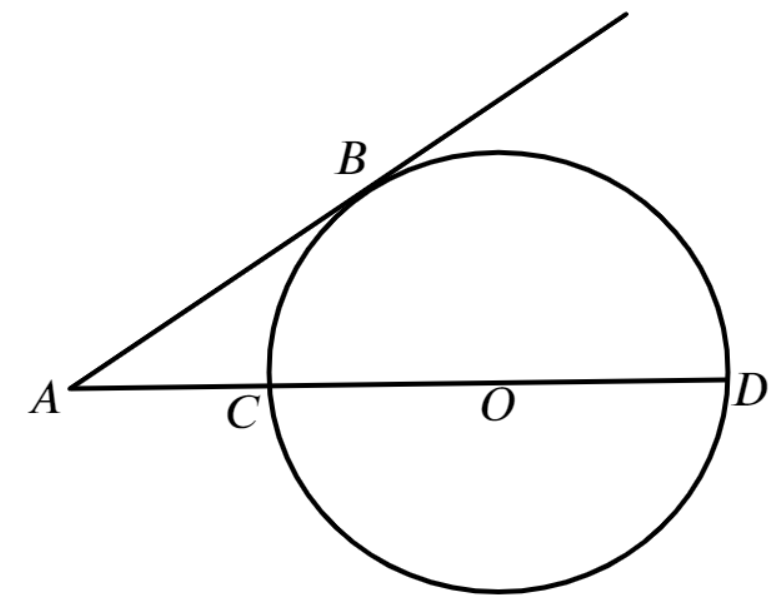
\includegraphics[scale=0.35]{g8-15.png}}
\end{figure}\\
По свойству касательной и секущей имеем $AB^2=AC\cdot AD.$ По условию $AD=2AB,$ значит $AB^2=AC\cdot2AB,\ AB=2AC.$ Пусть радиус окружности равен $x,$ тогда $AC=AD-2x,\ AC=2AB-2x,\ AC=4AC-2x,\ AC=\cfrac{2}{3}x.$ Поэтому $AB=2AC=\cfrac{4}{3}x.$\\
